\documentclass[11pt,a4paper]{ivoa}
\input tthdefs

\title{EPN-TAP: Publishing Solar System Data to the Virtual Observatory}

% see ivoatexDoc for what group names to use here
\ivoagroup{SSIG}

\author{Baptiste Cecconi}
\author{Stéphane Erard}
\author{Pierre Le Sidaner}
\author{Whoever Else}

\editor{Baptiste Cecconi}

% \previousversion[????URL????]{????Funny Label????}
\previousversion{This is the first public release}
       

\begin{document}
\begin{abstract}
???? Abstract ????
\end{abstract}


\section*{Acknowledgments}

???? Or remove the section header ????

\section*{Conformance-related definitions}

The words ``MUST'', ``SHALL'', ``SHOULD'', ``MAY'', ``RECOMMENDED'', and
``OPTIONAL'' (in upper or lower case) used in this document are to be
interpreted as described in IETF standard RFC2119 \citep{std:RFC2119}.

The \emph{Virtual Observatory (VO)} is a
general term for a collection of federated resources that can be used
to conduct astronomical research, education, and outreach.
The \href{http://www.ivoa.net}{International
Virtual Observatory Alliance (IVOA)} is a global
collaboration of separately funded projects to develop standards and
infrastructure that enable VO applications.


\section{Introduction}

???? Write something ????

\subsection{Role within the VO Architecture}

\begin{figure}
\centering

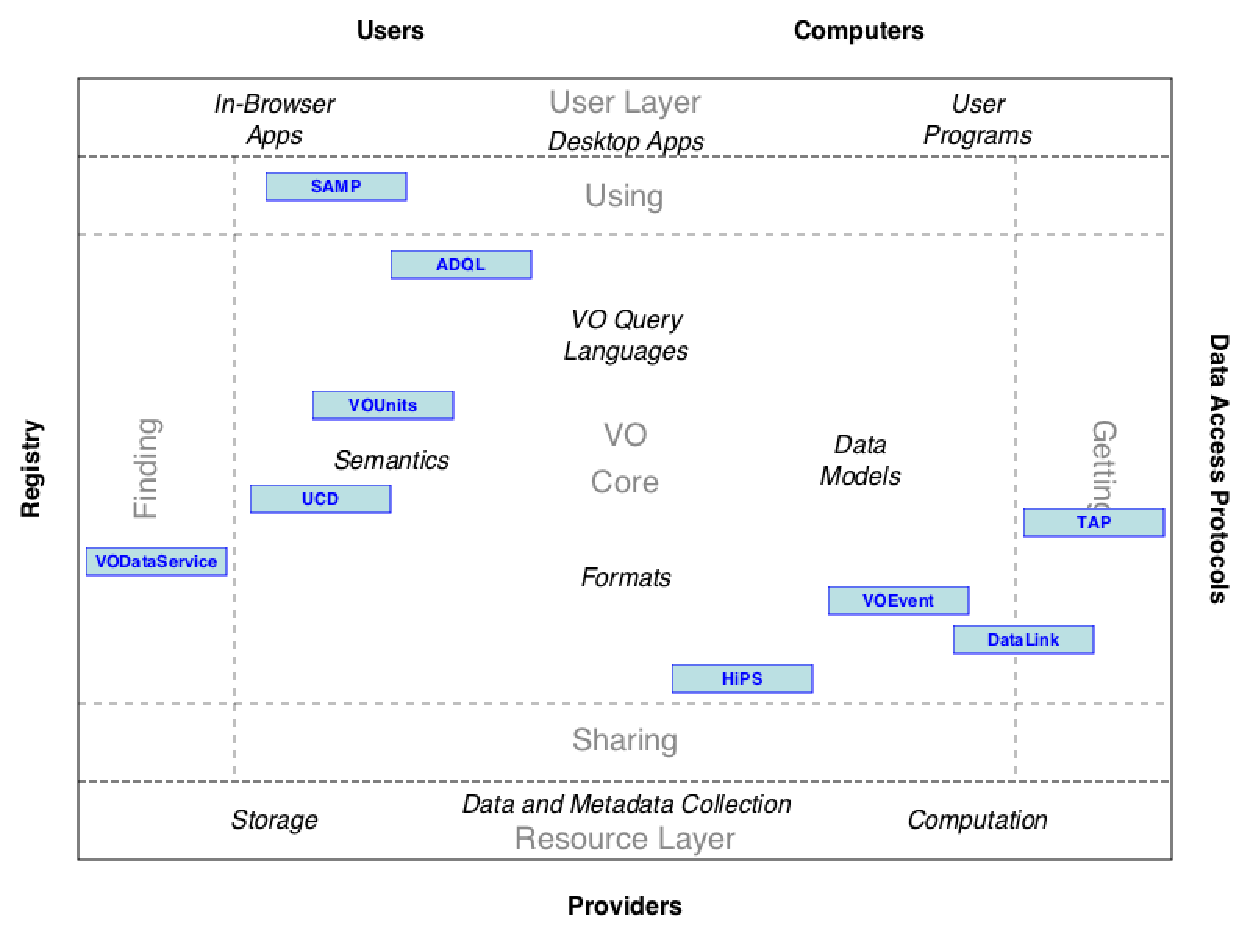
\includegraphics[width=0.9\textwidth]{role_diagram.pdf}
\caption{Architecture diagram for this document}
\label{fig:archdiag}
\end{figure}

Fig.~\ref{fig:archdiag} shows the role this document plays within the
IVOA architecture \citep{note:VOARCH}.

\section{The EPN-TAP Table Structure}

???? Prose ????

% GENERATED: python parse_source.py
\subsection{Europlanet2020-RI/VESPA Discussions Board}

\subsection{EPN-TAP v2 parameter description}

\subsection{Mandatory parameters}

\subsubsection{Mandatory parameters}

\paragraph(granule_uid)

Unique granule ID in data service.None

There can be only one file associated to a granule (plus possibly a thumbnail for quick-look purpose in a search interface).None

\paragraph(granule_gid)

Common to granules of same type (e.g. same map projection, or geometry data products) - think of it as a simple and convenient way to group or differentiate types of data.None

When several files relate to the same data, this parameter helps distinguishing them. This will allow the user to select the type of data of interest. E. g., a service may provide links to calibrated images, plus raw data and ancillary information for every granule; these will share the same obs_id, but will have different granule_gid.None

\paragraph(obs_id)

Associates granules derived from the same data (e.g. various representations / processing levels). May be the ID of original observation.None

\subsubsection{Mandatory parameters}

\paragraph(dataproduct_type)

The dataproduct_type parameter describes the high level scientific organization of the data product linked by the access_url parameter (see below), or directly included in the table (in which case the value is most likely 'ca' for catalogueNone). EPNCore currently defines several types listed below. The data provider must select the type most adapted to his data. In complex situations (e. g., when a file contains several data products), several types can be used to describe the same granuleNone — although using several granules to describe the file content may be a better solution. \\
 In the epn_core view these types are identified by a 2-characters ID, so that multivalued queries are unambiguous. Possible IDsNone are listed below with their meaning:None

\\
NoneNone

im \textbf{None}(= image): scalar field with two spatial axes, or association of several such fields, e.g., images with multiple color planes, from multichannel or filter cameras. Preview images (e.g. map with axis and caption) also belong here.None Conversely, all vectorial 2D fields are described as catalogue (see below). \\
None\item None
ma \textbf{None}(= map): scalar field / rasters with two spatial axes covering a large area and projected either on the sky or on a planetary body, associated to a Projection parameter (with a short enumerated list of possible values). This is mostly intended to identify complete coverages that can be used as reference basemaps. Does this require a secondary UCD notation (e.g., ;map)?\\
None\item None
sp \textbf{None}(= spectrum): measurements organized primarily along a spectral axis, e.g., radiance spectra. This includes spectral aggregates (series of related spectra with non-connected spectral ranges, e.g., from several channels of the same instrument - TBC).\item None
ds \textbf{None}(= dynamic_spectrum): consecutive spectral measurements through time, organized primarily as a time series. This typically implies successive spectra of the same target / field of view.\item None
sc \textbf{None}(= spectral_cube): sets of spectral measurements with 1 or 2D spatial coverage, e.g., imaging spectroscopy. The choice between image and spectral_cube is dictated by the characteristics of the instrument (which dimension is most resolved &amp; which dimensions are acquired simultaneously). The choice between dynamic_spectrum and spectral_cube is related to the uniformity of the field of view.\item None
pr \textbf{None}(= profile): scalar or vectorial measurements along 1 spatial dimension, e.g., atmospheric profiles, atmospheric paths, sub-surface profiles, traverses…\item None
vo \textbf{None}(= volume): other measurements with 3 spatial dimensions, e.g., internal or atmospheric structures, including shells/shape models (3D surfaces).\item None
mo \textbf{None}(= movie): sets of chronological 2D spatial measurements\item None
cu \textbf{None}(= cube): multidimensional data with 3 or more axes, e.g., all that is not described by other 3D data types such as spectral cube or volume. This is mostly intended to accommodate unusual data with multiple dimensions.\item None
ts \textbf{None}(= time_series): measurements organized primarily as a function of time (with exception of dynamical spectra and movies, i.e. usually a scalar quantity). Typical examples of time series include space-borne dust detector measurements, daily or seasonal curves measured at a given location (e.g. a lander), and light curves.\item None
ca \textbf{None}(= catalogue): applies to a single granule providing a list of events, a catalog of object parameters, a list of features... &quot;Spatial vectors&quot; (e.g., vector information from a GIS, spatial footprints…) belong here. This is relevant, e. g., for collections of vectorial elements (e.g. crater lists or ROI definitions) which can be handled directly in a specialized environment such as a GIS. This includes maps of vectors, e.g., wind maps.\\
None\item None
ci \textbf{None}(= catalogue_item): applies when the service itself provides a catalogue, with entries described as individual granules. The service can be, e. g., a list of asteroid properties or spectral lines. Catalogue_item can be limited to scalar quantities (including strings), and possibly to a single element. This organization allows the user to search inside the catalogue from the TAP query interface.None\item None
ev\textbf{None} (= event): introduce VOevents formatted according to IVOA Nonestandard (or possibly eventsNone with other formatting, TBC)\\
None\item None
\begin{itemize}None\end{itemize}
\\
NoneNone

Usage:None\\
None\emph{None}\emph{None}select\emph{None}None *\emph{None}None from\emph{None}None epn_core\emph{None}None where dataproduct_type like 'im'\emph{None}None\\
or \\
select *\emph{None}None from\emph{None}None epn_core\emph{None}None where i\emph{None}Nonevo_hashlist_has(lower(dataproduct_type\emph{None}None), 'im') =1\\
 will return only image data (the second syntax handles lists of values)\\
NoneNone

\paragraph(measurement_type)

The measurement_type parameter defines the physical quantities contained in the data, using UCDs. It relates to the reported quantity, not to the type of experiment. Therefore only UCD related to physical quantities can be used; e.g., phys.absorption;em.opt.I is eligible, while stellar_occultation is not. \\
 The provider must use the &quot;UCD1+&quot; list from IVOA as a reference, and should extend it only when necessary [RD8]:\\
 http://www.ivoa.net/Documents/REC/UCD/UCDlist-20070402.pdfNone\footnote{TODO:URL here}None \\
 The measurement_typeNone parameter is used to search data relevant to a certain field. Whenever several quantities are comprised in the granule, the measurement_type parameter must therefore refer to all these quantities, including multiple UCDs if needed.\\
Quantities derived from modeling/simulationNone are described by the regular UCD with &quot;;meta.modelled&quot; appended.\\
 Extra UCDs will be proposed/requested to IVOA. In the meantime, an extended list of UCDs will be made available in the EPN-DM document (in progress). \\
 Examples:None\\
 For images in general (i.e. actual measurements with a camera), the relevant UCD is obs.imageNone, whatever the calibration level.\\
 For spectra phot.flux.densityNone describes a flux\emph{None} vector (irradiance), while radiance and reflectance are not really definedNone currently (the closest UCDs are phys.luminosity;phys.angArea;em.wl and phys.albedo).\\
The associated spectral vector is described by UCDs em.wl, em.freq or em.energy, and the related error is described by stat.error;phot.flux.density (for flux).None

\paragraph(processing_level)

In the framework of EPN-TAP, this parameter is intended to provide the user with a quick evaluation of data &quot;usability&quot;. Several classifications are in use in different contexts, as summarized in the table below.  EPNCore v2 uses the CODMAC levels / PDS3 but removes the intermediate calibration levels; this is equivalent to using the simplified PDS4 levels and maintaining a separated level for ancillary data {reason for this: level 4 is used in only 2 services by the end of 2016, and wrongly; this was also a strong suggestion from the reviewers of the 2014 paper}.None &quot;Partially calibrated&quot; datasets are in general considered as not calibrated, but this evaluation is up to the data provider depending on context. &quot;Ancillary&quot; data include all extra information documenting the measurements, in particular coordinates or geometry files. Although it may be more consistent to separate calibration levels in different data services, several levels can be included in the same service (in particular calibrated and ancillary data). Only one value can be accommodated in this field, so the most advanced level (1-5) must be used whenever several levels are available in the same granule (TBD: use list instead?)None

Most EPN_TAP data services are expected to include Calibrated or Derived data. Other values would therefore only flag associated products.\\
 \\
 (Compilation of information from PSA, PDS4, &amp; ObsCore documents)None

???????????????????????????None\\
EPN-TAP v2\textbf{None} level\textbf{None}None

None&CODMAC\textbf{None} level \textbf{None}None

/ EPN-TAP v1\\
\textbf{None}None

None&PSANone\textbf{None} level\textbf{None}None

None&NASA\textbf{None} level\textbf{None}None

None&PRODUCT_TYPE \textbf{None}None

(PDS3/PSA)\textbf{None}None

None&PDS4\textbf{None}None&ObsTAP\textbf{None}None

None&Description\textbf{None} \\
 (from\textbf{None} PSA, with comments)\textbf{None}None

None&None\\1 \\
\\
None

None&1 \\
 (raw)None

None&1aNone

None& None

None&UDRNone

None&TelemetryNone&Level 0None

None&Unprocessed Data Record \\
 (low-level encoding, e.g. telemetry from a spacecraft instrument. Normally available only to the original team)None

None&None\\2 \\
\\
None

None&2 \\
 (edited)None

None&1bNone

None&0None

None&EDRNone

None&RawNone&Level 1 \\
 (std data format)None

None&Experiment Data Record \\
 (often referred to as &quot;raw data&quot;: decommutated, but still affected by instrumental effects)None

None&None\\3 \\
\\
None

None&3 \\
 (calibrated)None

None&2None

None&1ANone

None&RDRNone

None&CalibratedNone&Level 2None

None&Reduced Data Record \\
 (&quot;calibrated&quot; in physical units)None

None&None\\5None

None&4 \\
 (resampled)None

None& None

None&1BNone

None&REFDRNone

None&DerivedNone& None

None&Reformatted Data Record \\
 (mosaics or composite of several observing sessions, involving some level of data fusion)None

None&None\\5 \\
\\
None

None&5 \\
 (derived)None

None&3None

None&2-5None

None&DDRNone

None&DerivedNone&Level 3None

None&Derived Data Record \\
 (result of data analysis, directly usable by other communities with no further processing)None

None&None\\6 \\
\\
None

None&6 \\
 (ancillary)None

None& None

None& None

None&ANCDRNone

None&DerivedNone& None

None&Ancillary Data Record \\
 (extra data specifically supporting a data set, such as coordinates, geometry…) NoneNone

None&None\\None\begin{tabular}None\end{tabular}

None

\subsubsection{Mandatory parameters}

\paragraph(target_name)

The target_name element identifies a target by name or ID. The target may be any Solar System body, exoplanet, planetary sample, or meteorite, plus in some cases astronomical objects or spacecraft. Any other feature (craters, regions, atmospheric layers…) must be named using the optional feature_name parameter (see 4.3.3). This parameter can be multivalued only to describe several targets related to a granule; alternative names of the same target can be provided through the optional alt_target_name parameter.\\
 The best practice is to use the official designation of the target as defined by IAU [RD19]. This parameter is case sensitive (mixing lower/upper cases) and all values must use the standard spelling and case. Data providers must be aware that services which do not use the IAU designations might not be accessible by the clients. Conversely, users must be aware that some services containing data of interest might not be visible, if they do not use the recommended IAU nomenclature for planetary bodies. The SSODnet name resolver provided by VOParis-IMCCE may help data providers (and users as well) to handle multiple denominations [RD11None].\\
Concerning celestial objects (at fixed position, i. e., stars, galaxies…) the name should be identifiable through Simbad (http://simbad.u-strasbg.fr/simbad/None\footnote{TODO:URL here}).None

Other best practicesNone are listed below: \\
 The Exoplanet Encyclopedia provides a complete list of currently known extrasolar planets:\\
 http://exoplanet.eu/None\footnote{TODO:URL here} \\
 Meteorite catalogs can be found here:\\
 http://www.nhm.ac.uk/research-curation/research/projects/metcat/search/indexsing.dsmlNone\footnote{TODO:URL here}\\
 http://www.lpi.usra.edu/meteor/index.phpNone\footnote{TODO:URL here} \\
 The catalog of lunar samples is available here:\\
 http://www.lpi.usra.edu/lunar/samples/None\footnote{TODO:URL here} \\
 Other planetary samples are listed in topical web sites, e.g. samples from the Stardust mission are described here:\\
 http://curator.jsc.nasa.gov/stardust/catalog/None\footnote{TODO:URL here} \\
Asteroids:\\
Usage is to use preferably name (if it exists) or principal designation (number is not used here, can be included in alt_target_name)\\
Calibration:\\
Values can relate to existing names in a given archive (e.g., the PSA contains values such as bias, checkout, dark, flatfield, internal source…)\\
 Usage:None\\
 select\emph{None}None *\emph{None}None from\emph{None}None epn_core\emph{None}None where\emph{None}None target_name like 'Ceres' or\emph{None}None target_name like 'Vesta'\emph{None}None and\emph{None}None target\emph{None}None _type like 'dwarf_planet'\emph{None}None or\emph{None}None target_class like 'asteroid'\emph{None}None \\
 Will returnNone dataNone onlyNone fromNone 1None CeresNone orNone 4None Vesta (see ADQL syntax). Complex queries may also include parenthesesNone \\
 ExampleNone\\
 1P is the official IAU designation for comet Halley.\emph{None}NoneNone

\paragraph(target_class)

The target_class element identifies the type of a named target. A target is defined without ambiguity by a couple of parameters: target_class and target_name (although some targets may have no proper name). \\
 EPNCore defines the possible values for target_class: \\
 asteroid, dwarf_planet, planet, satellite\\
 (types from IAU list [RD22])\\
 comet, exoplanet, interplanetary_medium, ringNone, sample, sky, spacecraft, spacejunk, star, calibration \\
 (extra types defined for EPN)None \\
 Usage:None\\
 Any target has a unique target class.\\
 &quot;interplanetary_medium&quot; refers in particular to interplanetary dust.\\
 &quot;sample&quot; refers to lunar or planetary samples, to meteorites, but also to terrestrial samples, e.g., in laboratory studies.\\
 &quot;satellite&quot; stands for natural satellites only - other cases are handled though spacecraft or spacejunk.\\
 &quot;star&quot; is used typically for calibration targets, and for the Sun.\\
 &quot;sky&quot; may be used for other celestial bodies, usually referred to by their sky coordinates. It also includes the Interstellar Medium.\\
&quot;calibration&quot; is used for observations only related to instrument or signal calibration, including dark current, flat field, reference sample (in lab), etc.NoneNone

Comment\emph{None}: SsODNet uses &quot;Types&quot; of objects which are all included in EPN-TAP list: &quot;Asteroid&quot;,&quot;Spacecraft&quot;,&quot;Comet&quot;,&quot;Exoplanet&quot;,&quot;Spacejunk&quot;,&quot;Satellite&quot;,&quot;Planet&quot;,&quot;Dwarf Planet&quot;,&quot;Star&quot;\\
Additional EPN-TAP classes are: interplanetary_medium, ring, sample, sky, calibration \\
NoneNone

\subsubsection{Mandatory parameters}

\paragraph(time (min/max))

The time_min and time_max parameters provide the date and time of acquisition in the observer frame. NoneNone

In EPN-TAP, the time parameters are always provided in UTCNone and formatted in Julian daysNone (expressed as a double precision float). Although ObsCore uses Modified JD, EPNCore uses standard JD to avoid ambiguity with time origin. With double precision floats, the accuracy is on the order of 1 ms, which is considered sufficient to identify data of interest (the initial accuracy is preserved in the data itself).\\
 The two values min/max permit to handle long periods. Whenever acquisition time is a scalar (rather than an interval), both time_min and time_max must contain the same value in the table. There is no limiting value to this parameter.\\
 Examples:None\\
 http://&lt;server\emph{None}None address&gt;/tap/sync/request=doquery &amp; lang=adql &amp; query=select\emph{None}None *\emph{None}None from\emph{None}None epn_core\emph{None}None where\emph{None}None time_min &gt;\emph{None}None '2455197.5'\emph{None}None and time_max &lt; '2455927.5'\emph{None}None \\
 Will search data described by a time rangeNone \\
 http://&lt;server\emph{None}None address&gt;/tap/sync/request=doquery &amp; lang=adql &amp; query=select\emph{None}None *\emph{None}None from\emph{None}None epn_core\emph{None}None where\emph{None}None time_min between\emph{None}None '2455197.5' and '2455927.5'\emph{None}None \\
 Will search data described by a start time parameterNoneNone

Time range is normally provided in the observer frame (i.e., at the observer location), which is almost always the native time in the data. For instance, space-borne observations are usually documented with spacecraft on-board time, which is expected here (provided as JD, not as on-board clock timing). For other cases, the location where time is measured must be provided though the time_origin parameter (see section 8).\\
To support space-borne vs ground-based campaigns, multiple spacecraft observations, or survey of periodic events, measurement times need to be corrected for light path. Whenever comparisons are potentially involved, the use of the target_time_min and target_time_max parameters is recommended in addition to time_min and time_max to simplify this kind of comparison.\\
Non-compulsory parameters may be used to accommodate additive, specially formatted time scales such as native on-board time (see section 8). The information of the time_min and time_max parameters is however greatly recommended for observations, as it is used by default to search datasets.None

\paragraph(time_sampling_step (min/max))

These parameters provide the sampling step for measurements of dynamical phenomena, and for computations. This is the time between 2 successive measurements or data, which is mostly relevant when the measurements are regularly spaced. This may also be used as an input parameter, e.g., for ephemeris computations. \\
 This parameter is intended to allow the user to search for time-resolved observations of dynamic phenomena.None

\paragraph(time_exp (min/max))

These parameters correspond to the integration time (or exposure time) of measurements. It provides an estimate of the time resolution for dynamical phenomena, as well as an indication of relative S/N ratio inside a given dataset. This time is usually shorter than the time_sampling_step if both are present. It provides the overall integration time, i.e. individual exposure time x number of summed frames when relevant. NoneNone

\paragraph(spectral_range (min/max))

The spectral_range parameters define the upper and lower bounds of the spectral domain of the data. As mentioned previously, this quantity is conventionally expressed on a frequency scale in Hertz. Conversions to the native unit are provided in Appendix A.\\
Since this is the standard parameter to identify a spectral location, it is recommended to fill it even for images obtained through a filter. \\
 The spectral range and associated parameters only apply to electromagnetic waves. See the optional parameters particle_spectral_* for particle energy or mass detection.None

\paragraph(spectral_sampling_step (min/max))

The spectral_sampling_step parameters provide the spectral separation between the centers of two adjacent filters or channels. Like all spectral_* quantities, it is expressed on a frequency scale in Hz. Conversions to the native unit are provided in Appendix A. NoneNone

These parameters are mostly intended to provide an order of magnitude, e.g., to distinguish between grating spectrometers and Fourier spectrometers, or between observations related to surfaces or atmospheres. It can also help distinguishing between Nyqvist and sub-Nyqvist sampling rates.None

\paragraph(spectral_resolution (min/max))

The spectral_resolution parameters correspond to the spectral bandwidth used for the measurement (Full Width at Half Maximum). In case of a filter camera this is the filter bandwidth; in case of a spectrometer this is the spectral resolution per se. \\
 These parameters are mostly intended to provide an order of magnitude, e.g. to distinguish between grating spectrometers and filter cameras.None

Practical computation can be performed as  (c = 2.99792458E8):\emph{None}\\
df = c*1E6 dlam / lam^2 (from wavelength, with lam and dlam in micron)\\
df = c*1E3 dlam / lam^2 (same if dlam provided in nm)\\
df = c/1E-2 du (from wavenumber u in cm-1)NoneNone

\paragraph(c1 (min/max))

\paragraph(c2 (min/max))

\paragraph(c3 (min/max))

These parameters provide up to three spatial coordinates of the measured target. The coordinates depend on the spatial frame type defined below. All services must handle three spatial coordinates, even if the third one is always set to NULL. NoneNoteNone that the c3 parameter is related to the observed area; the target distance (e. g., geocentric distance for ground based observations, or spacecraft distance) is introduced by the optional parameter &quot;target_distance&quot;.NoneNone

In order to make uniform requests possible, spatial coordinates provided in the epn_core view must be standardized. However, they can be provided in several systems types, as defined by the spatial_frame_type parameter. \\
The native coordinate system used with the dataset can be described by parameters spatial_coordinate_description and spatial_origin. This is intended to provide this information prior to loading the data, especially when several coordinate systems are available in the same service. Descriptions for EPN-TAP are provided in [RD17]. \\
 Secondary coordinates can be introduced in the view using additional parameters, e.g., c1 and c2 providing central longitude and latitudeNone of a planetary disk, and extra RA / DEC columns providing location on the sky at this moment.None

\paragraph(c1_resol (min/max))

\paragraph(c2_resol(min/max))

\paragraph(c3_resol(min/max))

These parameters provide a simple estimate of resolution, either the FWHM of the PFS on the sky (in degrees), or the pixel size on a surface (in m), depending on spatial_frame_type. \\
 The client front-end may propose more appropriate units to the user, depending on context (e.g., angular resolution in mas, distance in m…).None

\paragraph(spatial_frame_type)

Provides the &quot;flavorNone&quot; of the coordinate system, which defines the nature of the spatial coordinates (c1,c2,c3) in the epn_core view and queries, and the way they are defined. This may be different from the coordinate system associated to / included in the data themselves. A value is required (use &quot;none&quot; if not applicable, &quot;body&quot; may also be OK in most casesNone). The possible types are described below: \\
 celestialNone\textbf{None}:None 2D angles on the sky, i. e. , right ascension c1 and declination c2 + possibly heliocentric distance in c3 – although this is a special case of spherical frame, the order and conventions are different. Earth distance may be provided as target_distance whenever relevant (ground-based observations). Assumes ICRS coordinates; right ascension is provided in degrees.\\
 body:\textbf{None} 2D angles in body-fixed frame: longitude c1 and latitude c2 + possibly altitude (above a reference surface) as c3. (c3 is expected to only provide an order of magnitude in general, not to be a fine search parameter)\emph{None}\\
Planetocentric system with eastward longitudes in the range (0,360)° is expected. Current IAU frame is assumed, in particular for definition of  prime meridian.\\
IAU 2009 planetocentric convention [RD12] applies, in particular eastward longitudes and a north pole located on the north side of the invariant plane of the Solar System for planets and satellites (see [RD12] for small bodies, and Annex A for details).  None\emph{None}\\
 The spatial_coordinate_description and spatial_origin attributes allow the data provider to indicate different conventions, e. g., to indicate a planetographic frame, or to use altitude above a reference surface as the third coordinate. It is stressed however that using other frames will make comparisons between datasets more difficult.\\
- No, that would preclude uniform queries. These 2 param have to relate to the coordinates provided with the data.\\
\emph{None}None

- Two other parameters are available to provide other vertical scales, see below (radial_distance and altitude_fromshape). \\
- Planetary interiors have C3 &lt;0 \\
- Planetocentric rotating frames are defined as spherical (TBC)\\
NoneNone

cartesian:\textbf{None} (x,y,z) as (c1,c2,c3). This includes spatial coordinates given in pixels.\\
 spherical:\textbf{None} (r, theta, phi) as (c1,c2,c3), as defined in ISONone standard None\footnote{TODO:URL here}80000-2:2009None\footnote{TODO:URL here}; r = radius; theta = zenith angle/colatitude/inclination; phi = azimuth (E longitude). Angles are provided in degrees. When related to the sky or to a solid body, &quot;celestial&quot; (with RA/Dec) or &quot;body&quot; (with longitude/latitude) coordinates must be used instead. \\
cylindrical:\textbf{None} (r, theta, z) as (c1,c2,c3); r = radius; theta = azimuth; z = height. The angle is provided in degrees.\\
none:\textbf{None} to be used when no spatial frame is defined for the dataset. This is intended to prevent useless searches when space coordinates are not defined (a non-zero value is required by the mixin).None

spatial_origin\emph{None} used to indicate center of frame ?None

Not used in the view (only possible in the data) ?\emph{None}\\
 healpix:\textbf{None} TBC (Nside and pixel#? Should also specify or assume ordering (nested/ring) ) - TBC, wait for IVOA decision.NoneNone

\\
 This parameter, although related to the specific coordinate system in use, is mostly intended to identify the nature of the coordinates handled by the service (e. g., angles versus distances).\\
 This parameter is provided as a column of the epn_core view, to ensure it can be queried through the basic TAP mechanism. Although it will in general remain constant along the table for simple services, this parameter can vary from granule to granule and a value must therefore be provided in any query that includes spatial coordinates. Whenever additional coordinates are provided, they must be stored in extra columns of the table. If several different frames are mixed to provide the main coordinates, the use of different granule_gid may help clarify the situation. At any rate, easy access to the data must be considered during the design of the service. \\
 Ranges and specific definitions vary with the actual frame in use, and are discussed in Appendix A. - Only applies to the system provided in the data?None\emph{None} NoneNone

\paragraph(incidence_angle (min/max))

The incidence angle parameters define the upper and lower bounds of the incidence angle variation in the data (also known as Solar Zenith Angle). This is always indicated in decimal degrees, and may range from 0 to 90° (with 0° indicating the normal to the surface).\\
 Incidence and emergence angles may be counted relative to the normal of the ellipsoid model, or to the local normal (e. g., using a 3D shape model). In case the two systems are included in the data, these keywords introduce the values relative to the ellipsoid (local values may be available through non-compulsory parameters).None

\paragraph(emergence_angle (min/max))

The emergence angle parameters define the upper and lower bounds of the emergence angle variation in the data (viewing angle). This is always indicated in decimal degrees, and may range from 0 to 90° (with 0° indicating the normal to the surface).\\
 Incidence and emergence angles may be counted relative to the normal of the ellipsoid model, or to the local normal (e. g., using a 3D shape model). In case the two systems are included in the data, these keywords introduce the values relative to the ellipsoid (local values may be available through non-compulsory parameters).None

\paragraph(phase_angle (min/max))

The phase angle parameters define the upper and lower bounds of the phase angle variation in the data (scattering angle - 180°, or angle light source-target-observer). This is always indicated in decimal degrees, and may range from -180 to 180° (with 0° corresponding to opposition, i. e., light source in the back of the observer). Negative values may refer, e. g., to geometry before opposition, depending on context.\\
 Phase, incidence and emergence are partly related:\\
 abs(i - e) &lt; phi &lt; i + e\\
 If the azimuth angle a is provided instead of the phase angle, the latter can be derived from knowledge of the three angles:\\
 cos phi = cos i cos e + cos a sin i sin eNone

\paragraph(s_region)



Another mandatory parameter provides additional information about axes coverage.None

This parameter introduces a footprint for spatially extended data products in 2D, most notably on the sky (using RA, Dec) or on planetary surfaces (using E longitude, latitude). This is a single parameter with no min/max declinations. It must contain a PgSphere spoly variable with syntax: '{(lon1,lat1), (lon2,lat2), … }' (with no quotesNone) where (lon1,lat1)None = (10.d, 5d), character d included (for degrees). Pairs (lon1,lat1) must sample the dataproduct contour in sequence, provided in direct (counter-clockwise) senseNone.None The result of the query is an STC-S string (as in ObsCore; currently retrained to polygons).\\
NoneNoneNone

In addition, the resource descriptor (q.rd for DaCHS) must contain the line (for body coordinates):NoneNoneNone




&lt;stc&gt;  Polygon UNKNOWNFrame [s_region] &lt;/stc&gt;egin{verbatim}None\end{verbatim}


None



None

None

\\
NoneNoneNone

Open issue: this work directly in celestial coordinates, using ICRS as POLYGON value. On a planetary body, frame UNKNOWNFrame must be used. The difficulty is that W longitudes are assumed in this case. To be discussed at IVOANone. NoneThe recommendation is to build s_region contours using W longitudes for the time being, but this will change in the future.NoneNone

\subsubsection{Mandatory parameters}

\paragraph(instrument_host_name)

This parameter provides the name of the observatory or spacecraft that performed the measurements. The best practice is to use names from the lists indicated below. A list of host names must be provided for integrated data sets. \\
 For ground-based observations, the reference is the list of IAU observatory codes: http://www.minorplanetcenter.net/iau/lists/ObsCodesF.htmlNone\footnote{TODO:URL here}\\
 However, this list is not intended to include all ground-based observatories, and a complement still needs to be identified (including e. g. radio-telescopes).\\
 A reasonably complete list of radio-telescopes is available here: \\
 http://en.wikipedia.org/wiki/List_of_radio_telescopesNone\footnote{TODO:URL here}None

Other open Q:None

are IAU ID eligible?\item None
granularity is very heterogeneous (e.g. one single entry for Paranal or Mauna Kea, but many for Siding Spring).\item None
\begin{itemize}None\end{itemize}
Some entry related to obs programs (New Horizon KBO search from various sites) \\
 Concerning space-borne data, the most complete list of international planetary missions and orbital observatories is found here (included in a complete list of space missions with ID):\\
 http://nssdc.gsfc.nasa.gov/nmc/None\footnote{TODO:URL here}\\
 Planetary missions are also listed here:\\
 http://nssdc.gsfc.nasa.gov/planetary/chronology.htmlNone\footnote{TODO:URL here} \\
 Alternatively, the PDS dictionary defines values for many mission names:\\
 http://pds.nasa.gov/tools/dictionary.shtmlNone\footnote{TODO:URL here}\\
 Other mission names are supported by the SPICE system, but only as ID codes:\\
 http://www-int.stsci.edu/~sontag/spicedocs/req/naif_ids.htmlNone\footnote{TODO:URL here}\\
 (TBC – Spice is unambiguous but only uses IDs, PDS values are explicit but somewhat arbitrary)\\
 In the epn_core view, the acronym is preferred to the full name to avoid long strings and related errors. Both values can be provided (e.g., HST + Hubble Space Telescope).None

\paragraph(instrument_name)

Identifies the instrument(s) that acquired the data. A list of instruments must be provided for integrated datasets. \\
 Service providers are invited to include multiple values for instrument name, e.g., complete name &amp; usual acronym. This will allow queries on either &quot;VISIBLE AND INFRARED THERMAL IMAGING SPECTROMETER&quot; or &quot;VIRTIS&quot; to produce the same reply. They must be separated by the # character to be queried.\\
Example:\emph{None}\emph{None}\\
VISIBLE AND INFRARED THERMAL IMAGING SPECTROMETER#VIRTIS\emph{None}NoneNone

Concerning space-borne data, the most complete list of international planetary missions and orbital observatories is found here:\\
 http://nssdc.gsfc.nasa.gov/nmc/None\footnote{TODO:URL here}\\
 Instruments on board planetary missions in particular are listed here:\\
 http://nssdc.gsfc.nasa.gov/nmc/experimentSearch.doNone\footnote{TODO:URL here}None

 None

\subsubsection{Mandatory parameters}

\paragraph(service_title)

Provides an acronym for the service/table title. This is used to refer to the service providing the data, therefore this must be identical to the name of the schema and must be constant in the view.\\
When designing the service, care should be taken to use a schema name not already ascribed to another EPN-TAP service.None

\paragraph(creation_date)

Provide the date when the granule was introducedNone

\paragraph(modification_date)

Provide the date when the granule was last updated (intended to speed up mirroring between sites)None

\paragraph(release_date)

Provide the date when the granule becomes public (intended to preserve proprietary period, usage TBD)None

\subsection{Optional parameters}

\subsubsection{Optional parameters}

\paragraph(access_url)

The data of interest are often stored in a file, not in the table itself. In this very usual case, the access_url parameter provides a complete path to the data products on the network, so that they are accessible for download by plotting or processing tools. All URLs in the epn_core view are case sensitive and must provide an actual link. However, the link may be the output of a script on the server, in which case this parameter provides a call to the script with adequate arguments (e.g. Titan atmospheric profiles service). In any case, this parameter must link to the actual data, not to a file of metadata nor to a document.\\
 Whenever the data consists in a few scalar fields, this parameter may be replaced by parameters providing the data itself (e.g. mass, in a table providing the masses of Solar System bodies).None

\paragraph(access_format)

Access_format provides the format of the data file linked through the access_url parameter. \\
 The data may be stored in their native format, and no format conversion is required to set up an EPN-TAP service. This field can therefore include reference to unusual formats, although those may not be handled by plotting tools but only in a specific environment. Consistently with ObsCore, possible values are MIME-types written in lower cases and are listed in Appendix F (Data Formats and MIME TypesNone\footnote{TODO:URL here}).None

\paragraph(access_estsize)

The access_estsize field provides an order of magnitude (in kilobytes) of the file available via the corresponding URL. It is intended to provide an indication that can help to tune download functionalities in an application, depending on data volume and transfer bit rate.None

\\
None

• OtherNone parameters may be used to describe the data files:\textbf{None}None

\paragraph(thumbnail_url)

The thumbnail_url parameter contains the URL of a reduced version of the data product used for quick-look purpose (e.g., a small jpeg image, typically 200x200 pixels). This may be handy in the case of big data files or unusual data formats, to facilitate data selection by the user. The EPN-TAP client uses this thumbnail for on-line quick-look, which therefore provides important added value to a service. Preferred formats include jpeg and png, which are handled easily by a basic viewer. Larger or more elaborate previews can be provided as independent granules and identified via a granule_gid different from that of the data. All URLs in the epn_core view are case sensitive and must provide an actual link.None

\paragraph(file_name)

The file_name parameter introduces the name of the data\emph{None} file, with extension but no path information. In many data services, the file name encodes the most relevant metadata and may be a very handy access mechanism for specialists. In services providing sets of files in a complicated directory tree (e.g., related to a spacecraft operation plan), the file_name parameter is a handy key to perform automatic operations such as mirroring, pipeline processing, etc - a web service is available to retrieve a file from the file_name parameter in any EPN-TAP service (File grabbing interfaceNone\footnote{TODO:URL here}). Its use is therefore always recommended when data are provided in separated files, i. e., not included in the table.\\
All file_name values in the epn_core view are case sensitive and must reflect the filename of the product provided through access_url; for instance, if this is a link to script converting an ascii file to VOTable, file_name must refer to the outcome of this script, in this case the VOTable.None

\paragraph(access_md5)

This parameter introduces a MD5 Hash for the file when available (link to a real file), to be used as a checksum.\\
NoneNone

\paragraph(accref)

Not an EPN-TAP parameter, but apparently used to introduce an URL with datalink in TAP / DaCHS (present in epncore2 mixin) - really? Also seems required to access data files located on the same DaCHS server. See with developers Nonefor use in TOPCAT and VESPA portalNoneNone. May also be required to handle proprietary periods, TBCNone. \\
NoneNone

\paragraph(datalink_url)

This parameter is used to provide extra accesses through a datalink/SODA interface. It can either provide a table of hard links or a dialogue to setup input values and call a web service. Input values can be retrieved from the current granule; if several EPN-TAP parameters need to be passed, they must be concatenated in an extra parameter in the table (often called ds_id\textbf{None}). TBC: does this need to be called this way?None\\
NoneNone

 None

\subsubsection{Optional parameters}

\paragraph(solar_longitude (min/max))

Solar longitude (a.k.a. heliocentric longitude, or ecliptic longitude of the Sun, traditionally noted Ls) is the Sun-Planet vector angle counted from the planet position at N hemisphere spring equinox. It provides a measurement of season. \\
 Ls = 90° corresponds to the northern summer solstice, Ls = 180° to the northern autumn equinox, and Ls = 90° to the northern winter solstice. Although it is most usually applied to Mars and Titan (using Saturn's Ls), this notion can be enlarged to any planetary body without ambiguity.\\
 This should not be confused with the true anomaly of the body (which is the same angle counted from the perihelion position), nor with the longitude of the subsolar point (see below).None

\paragraph(local_time (min/max))

Planetary observations may be documented using the local time at the surface, i. e. the location of the solar meridian normalized to 24. This parameter is provided in unit of target rotation divided by 24 and is measured from local midnight (ranges from 0 to 24, must increase with time at a given location). It is provided in decimal hours.None

\paragraph(target_distance (min/max))

The target_distance parameter introduces the distance of the observer to the observed area (in km), not to be confused with a vertical dimension provided by c3. This is mostly intended for space borne data, where it provides the spacecraft-target distance in km. For ground-based observations the earth_distance parameter should be used instead (in au).None

\paragraph(target_time(min/max))

The target_time parameter introduces the time measured in UTC scale at the target. This is intended to correlate simultaneous observations such as ground-based support and space-borne observations, or mutlispacecraft campaigns.None

\paragraph(earth_distance (min/max)sun_distance (min/max))

For observational services, these two parameters provide the corresponding distance to the target at time of observation (in au).None

\subsubsection{Optional parameters}

\paragraph(subsolar_longitude (min/max))

\paragraph(subsolar_latitude(min/max))

Provide coordinates of sub-solar point, e.g., for ground-based observations.None

\paragraph(subobserver_longitude(min/max))

\paragraph(subobserver_latitude(min/max))

Provide coordinates of sub-observer point, in particular sub-Earth point (disk center) for ground-based observations.None

\subsubsection{Optional parameters}

\paragraph(ra (min/max))

\paragraph(dec (min/max))

If fixed sky coordinates of the target are provided in the view in addition to standard coordinates, they must be stored in parameters named ra and dec. This may document the location of a planet in a celestial image, while the main coordinates c1/c2 are used to describe the observed area as longitude and latitude. ICRS coordinate system is assumed; right ascension is provided in degrees (similar to ObsCore). RA, DECNone parameters are interpreted correctly by most VO tools.None

 NoneNone

\subsubsection{Optional parameters}

\paragraph(radial_distance (min/max))

Radio distance in km measured  from body centerNoneNone

\paragraph(altitude_fromshape (min/max))

Altitude from shape in km measuredNone from local surface, i.e. from the DTM or shape model at C1/C2)NoneNone

C3 can be used to select services/data in a given altitude range, while radial_distance and altitude_fromshape provide other convenient vertical scales to compare observations from various origins.\\
This use of C3min/max also applies for planetary interiors (C3 is then &lt;0) and measurements at high altitude/distance. \\
NoneNone

\subsubsection{Optional parameters}

\paragraph(Spatial_coordinate_description)

\paragraph(Spatial_origin)

These two parameters provide description of the spatial frame(s) in use, as introduced by the spatial_frame_type parameter. This is mostly relevant when this parameter is constant throughout the service.\\
 Possible values are detailed in [RD17], which is partly adapted from STC [RD13].None

Spatial_origin may be used to distinguish between altitude and distance from center when body coordinates are in use - TBC.\\
 ExamplesNone (TBC)\\
 BODY, Mars_IAU2000, \emph{None}ICRS\emph{None}None\\
Geocenter \emph{None}None \\
\\
None

\paragraph(time_origin)

This attribute states where the time is measured, and is expected to remain constant throughout the service. This knowledge is required to cross-correlate event-based observations, in particular to indicate light-path differences. It applies to the time_min and time_max parameters (target_time always refers to the target in the FoV). If this parameter is not informed, time is expected to be provided in the observer frame.\\
 Possible values for time_origin are:None

Earth, (solar system bodies), (spacecraft)\emph{None}NoneNone

\paragraph(time_scale)

Always UTCNone in data\emph{None} services (may be relaxed in computational services such as ephemeris) — from enumerated listNone.None

\paragraph(bib_reference)

The bib_reference parameter introduces an individual bibliographic reference at granule level. This may be required to provide the origin of the data, e. g., if the resource is a compilation of data from various origins.\\
 This is best provided as a bibcode (as used e. g. by ADS) or as a DOI. \\
A generic regular expression for bibcode (from IPDA discussions) is: None[0-9]{4}[A-Za-z0-9\&amp;\.]{5}[A-Za-z0-9\.]{9}[A-Z\.]\\
NoneSee Nonehttp://adsabs.github.io/help/actions/bibcodeNone\footnote{TODO:URL here}None

\paragraph(publisher)

Specifies the publisher of the data service\emph{None} (not necessarily at the origin of the data). Currently a free format string.\\
NoneNone

\paragraph(internal_reference)

The internal_reference parameter can be used to identify granules (or sets of granules) intimately related to the current one. E.g., in a service containing both observations and results of analysis of observation sets, internal_referenceNone can be used to provide the set of observations used to compute a result. This contains a list of granule_uid in the same service.\\
This is specifically intended to provide internal references in services which would otherwise need to be split in several tables, and should not be used in more usual cases. NoneNoneNone

\paragraph(external_link)

The external_link parameter can be used to provide extra information that does not fit easily in the view, and is intended for human reading only. This may be an extended discussion about a granule on a web site, which may include images, tables, or other documents. For instance, the individual planet pages of the Encyclopedia of exoplanets NoneNonecan be linked with this parameter. \\
NoneNoneNone

\paragraph(species)

The species parameter introduces the chemical species of interest in simple data services. The formatting is very basic and simply uses the standard formula in ascii, e. g., H2O for water, CO2 for carbon dioxide or Fe for iron. This is the only query parameter that is provided in case sensitive form, using the standard chemical notation. This format can only accommodate atoms and simple molecular species, and does not support isotopic variations. \\
 An example application is related to atmospheric composition: a table providing the vertical abundances of many gaseous species with altitude. All columns are abundances and are described by the same measurement_type parameter. Only the use of the &quot;species&quot; parameter (together with the column name itself) allows identifying the various species and accessing the requested information.\\
 If the data contain one column per species, it is recommended to also include the species in the column name (e.g., H2O_abundance). \\
 If more elaborated compositional information must be included, the use of another parameter providing InChiKeys is recommended - TBC (inChiKeyNone only related to molecule, including isotopes, but not physical state / phase; does not include #)\\
NoneNone

\paragraph(filter)

This parameter introduces the standard name of a filter used during measurements. This is reserved for filters in imaging mode (no grating/grism #, etc). There is no predefined list, because of the large variety of possible denominations, but the best practice is to use a short and accurate IDNone.\\
This is intended to document the results of a search, rather than a search parameter. Therefore, it is recommended to also fill the spectral_range_min/max parameters to describe filter imaging - this is the only way to make filter imaging easily searchable. None

\paragraph(alt_target_name)

This parameter introduces an alternative name of the target, especially when it is more usual than the official IAU one (e.g., Halley vs 1P).\\
Another possible usage is to store here a list of all alternative names of the target (e.g., for asteroids: name, number, principal and provisional designations).None

\paragraph(feature_name)

The feature_name parameter introduces a supplementary name to provide more details about the observed target. It is intended in particular to accommodate a local name (crater, surface feature, region name…) whereas target_name is reserved to describe the whole body (Mars, Moon, Ceres…). The best practice is to use the official features name defined by IAU [RD20] when relevant.\\
 The target_region parameter (see below) also provides additional information on the target, but is aimed at indicating the global scope of a database (e.g., atmospheric layer, internal structure…).None

\paragraph(target_region)

This parameter optionally identifies the region of interest for the resource, in complement to target_name. This parameter only introduces generic regions, not specific local names, which must be handled using the feature_name parameter (see examples above).\\
 The best practice is to take the values from standard sources:None

IVOA thesaurus: http://www.ivoa.net/rdf/Vocabularies/vocabularies-20091007/IVOAT/None\footnote{TODO:URL here}\item None
IAU thesaurus http://www.mso.anu.edu.au/library/thesaurus/None\footnote{TODO:URL here}\\
 + another version: http://www.vocabularyserver.com/trex/en/None\footnote{TODO:URL here}\\
 The latter seems more recent and more complete (although the interface is not practical)\item None
Spase dictionary http://www.spase-group.org/None\footnote{TODO:URL here}\\
ExampleNone: \\
&quot;atmosphere&quot;, &quot;surface&quot;, &quot;ionosphere&quot;\emph{None}None\\
 The same sources are used for the declaration file in the registry.\item None
\begin{itemize}None\end{itemize}
 None

\subsection{Extensions}

\subsubsection{Extensions}

\paragraph(particle_spectral_type)

This parameter and the following ones are related to the spectral distribution of particles only (see the spectral_* parameters for electro-magnetic waves).\\
 The particle_spectral_type parameter introduces the type of axis in use: either energy (provided in eV), mass (in amu), or mass/charge ratio (in amu/qe).None

\paragraph(particle_spectral_range (min/max))

The particle_spectral_range parameters define the upper and lower bounds of the spectral domain for particles. Depending on the particle_spectral_type parameter, this quantity is expressed on an energy, mass, or mass/charge scale, with respective units eV, amu, or amu/qe. \\
 Conversions to the native unit are provided in Appendix A.None

\paragraph(particle_spectral_sampling_step (min/max))

The particle_spectral_sampling_step parameters provide the spectral separation between measurements, in the same scale and unit as particle_spectral_range.\\
 Conversions to the native unit are provided in Appendix A. This parameter is mostly intended to provide an order of magnitude.None

\paragraph(particle_spectral_resolution (min/max))

The particle_spectral_resolution parameters correspond to the actual resolution of the measurements, and are provided in the same scale and unit as particle_spectral_range. \\
 This parameter is mostly intended to provide an order of magnitude.None

 None

\subsubsection{Extensions}

\paragraph(mean_radius)

\paragraph(equatorial_radius)

\paragraph(polar_radius)

parameters used to provide sizes (in km)\\
None

\paragraph(mass)

Mass in kgNone

\paragraph(sideral_rotation_period)

in hour\\
None

\paragraph(semi_major_axis)

in au,None

inclination, etc - to be reviewedNoneNone

See discussion page: orbital parametersNone\footnote{TODO:URL here}None

\\
When target_class = asteroid or dwarf_planet:\\
\textbf{None}None

\paragraph(dynamical_class)

introduces the class of small body, from enumerated list.\\
Includes: TNO, MBA, NEO - add OCC (Oort Cloud comet), JFC (Jupiter family comet) here, and Centaur, Trojan (but which planet?)None

\paragraph(dynamical_type)

introduces a subdivision of the above, from enumerated list\\
Currently includes: \\
NEO (complete): Atira, Aten, Apollo, Amor\\
TNO (complete, but check values): res 2:5 (develop?), res 1:2 (develop?), Plutino, Hot classical, Cold classical, Scattered disk object, Detached object, Inner Oort object (not strictly KBO?)\\
Values from MPC, unclear (as orbit_type): 4 NEO types + Object with perihelion distance &lt; 1.665 AU, Hungaria, MBA, Phocaea, Hilda, Jupiter Trojan, Distant Object, UnclassifiedNone

To be made consistent with SsODNetNone\\
\emph{None}\textbf{None}NoneNone

See discussion page: Small bodies sub-typesNone\footnote{TODO:URL here}None

\subsubsection{Extensions}

\paragraph(Projection)

parameter needed, list of values TBDNone\\
How do we define arguments / properties?NoneNone

 None

\subsubsection{Extensions}

\paragraph(original_publisher)

Services compiling data from many sources can use the original_publisher \textbf{None}parameter to refer to the source of the data.None

\paragraph(data_calibration_desc)

The \textbf{None}data_calibration_desc\textbf{None} parameter from the spectroscopy extension can be used to provide information on post-processing (preferably to a &quot;comment&quot; parameter)None

\paragraph(producer_name)

\paragraph(producer_institute)

ExperimentalNone data services may use producer_name\textbf{None} &amp; producer_institute\textbf{None}, etc - TBC\textbf{None}None\\
List TBD, see PVOLNone NoneNone

\\
NoneNone

\subsubsection{Extensions}

\paragraph(producer_name)

\paragraph(producer_institute)

provide reference to who measured the sampleNone

\paragraph(sample_classification)

provides composition as group, class, sub-class, etc… of sample concatenated in a hash-listNone (which allows for flexible searches with LIKE and %; this is in practice the only way to ensure that we get all results). Should include specification &quot;meteorite&quot; plus the meteorite type when applicable, as well as description of (main) mixtures ingredients. Meteorite types as in Krot et al 2005. Dana or Struntz classification tags can be used for minerals. Minor/trace components are not welcome here (would multiply false alarms).None

\paragraph(grain_size (min/max))

provide the particle size range in µm. A very large value (eg, &gt;1000 µm) can be used locally in a service to identify bulk material - see if we define a code for this (-1 could do, but we also have to reserve a code for N/A). This is really &quot;grain&quot;_sizNonee, since &quot;particle&quot; is reserved for particle spectroscopy above.None\\
NoneNoneNone

\paragraph(azimuth(min/max))

azimuth angle in degrees - see if negative values of angles can have a special meaningNoneNone

\paragraph(pressure)

\paragraph(temperature)

experimental conditions, in bar and KNone

The type of measurement/scale (REFF, I_over_F, etc…) is provided as a UCD through measurement_type\textbf{None} (to be defined in this case)None

• All *_desc\textbf{None} parameters introduce free descriptive strings in lower cases. They are not intended as search parameters (although they can be searched):None

\paragraph(sample_desc)

free string or hash-list describing the sample, its origin, and possible preparationNone

\paragraph(setup_desc)

free string or hash-list describing the experimental setup if needed - may include Aperture (size of sample measured), etcNone

\paragraph(data_calibration_desc)

free string or hash-list describing data post-processing / calibration (formerly processing_desc)None

\paragraph(geometry_type)

such as bidirectional, biconical, directional-hemispherical, etc - see if this list can be frozen (not likely)None

\paragraph(measurement_atmosphere)

description of experimental conditions, free string. Measurements under vacuum are indicated here with the word &quot;vacuum&quot;.None

\paragraph(thumbnail_url)

provides a link to a small spectral plot - caution should be taken to maintained minimal readability in small format in the VESPA portal. Larger plots can be included as separated granules.None

• External documents are often available to provide extra information in this context, e.g. chemical analysis or descriptive image of the sample. Such documents can be considered an extension of the table for the current granule, as opposed to other data products which must\emph{None} be defined as different granules/lines. The best solution identified consists in providing such links under the datalink_url parameter (as dlmeta)  - the alternative idea to use specific parameters such as Nonedocument_url, image_url… is deprecated.NoneNone

• More general parameters have restricted usage in this case:None

\paragraph(target_class)

target_class 'sample', constantNone

\paragraph(target_name)

provides an ID of the sample. It introduces the name of a meteorite or lunar sample when applicable. Various parts of the same sample can be indicated and described in sample_desc (such as &quot;Location A&quot;, etc).None

\paragraph(species)

species is also available, see if usage can be enlarged (e.g., to InChiKeysNone)None

• Other possible parameters, TBC:None

A parameter to identify a source database in a collective service (such as SSHADE)None

• Special cases to handle:None

Photometric measurement sets: some wlv and many angles, distributed togetherNone

Band lists: tables with characteristics and attributions - EPNCore may not be the best possible solution, TBCNone

Optical constants: ~ two associated spectra? or only one if complex data are available.NoneNoneNone

\\
None

\subsubsection{Extensions}

\subsubsection{Extensions}

\paragraph(access_url)

etc… are expected to link to a VOevent file (TBCNone) with dataproduct_type = ev ; access_format TBCNone (text/xml? or text/xml+voevent)None

\paragraph(instrument_host_name)

\paragraph(instrument_name)

Those parameters are expected to be &quot;simulation&quot; + code reference, including version number (or standard use if observations)None

for the time being:\textbf{None} put all targets involved as a list in target_name (e.g., Sun#Earth); use same obs_id to associate related eventsNone

 target_name \textbf{None}and time_min/max\textbf{None} describe the event location and time in all cases. Parameter event_mode\textbf{None} says if this is a source event or a consequence (if the event propagates). Related events (cause and consequences) have the same granule_gid.NoneNone

\textbf{}Alternatively\textbf{None}: event_origin_targetNone, event_origin_time\textbf{None}: provide location and time of an initial event. If the event propagates in the Solar System (usual case), target_name and time_min/max provide the location and place where effects are observed. Related events (cause and consequences) have the same granule_gid.NoneNone

\paragraph(event_type)

provides a type of event from a pre-defined list (e. g., meteor_shower…None)None

\paragraph(event_status)

distinguishes prediction, observation, and utility (e. g., local event related to an instrument, like a change of detector)None

\paragraph(event_cite)

can be &quot;followup&quot;, &quot;supersedes&quot; or &quot;retraction&quot;, TBCNone (alternative is to update the event lists)None NoneNone

\\
None

\subsubsection{Extensions}


% /GENERATED

\appendix
\section{Changes from Previous Versions}

No previous versions yet.  
% these would be subsections "Changes from v. WD-..."
% Use itemize environments.


\bibliography{ivoatex/ivoabib,ivoatex/docrepo}


\end{document}
